\graphicspath{{lectures/05_eloadas_abrak/}}

\section{5. előadás -- Szétválasztható egyenletek: zérushelyek, példák és visszavezethető típusok}

\subsection{A szétválasztható változójú egyenlet: a zérushelyek esete}
\textbf{Megjegyzés.} Tekintsük az
\begin{equation*}
    x'=g\cdot(h\circ x),\qquad x(\tau)=\xi
\end{equation*}
kezdetiérték-problémát. Az előző előadásban a $0\notin {R_h}$ esetet vizsgáltuk.

Mi a helyzet akkor, ha $0\in{R_h}$?

\textbf{1. példa.}
\[
    x'=x,\qquad x(\tau)=0
\]
globálisan egyértelmű.

\textbf{2. példa.}
\[
    x'=\sqrt{|x|},\qquad x(\tau)=0
\]
még lokálisan sem egyértelmű.

\textbf{Megjegyzés: improprius integrálok.}
\begin{align*}
\text{a)}\quad & \int_{0}^{1}\frac{1}{s}\,ds
    &&\text{divergens},\\
\text{b)}\quad & \int_{0}^{1}\frac{1}{\sqrt{s}}\,ds
    &&\text{konvergens}.
\end{align*}
\begin{center}
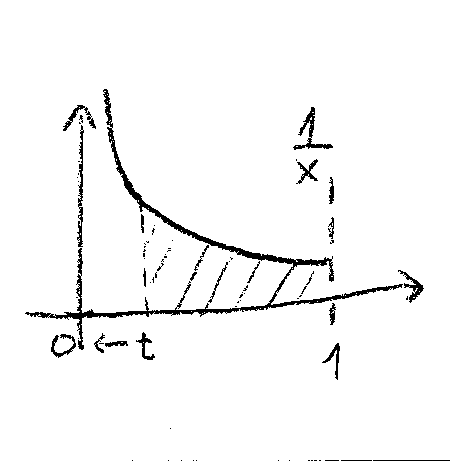
\includegraphics[width=0.27\linewidth]{improper_integral_01.png}
\figlabel{A $1/s$ függvény alatti terület szemléltetése a kéziratban (15. PDF-oldal).}
\end{center}

\noindent\textbf{Tétel.}
Legyen
\[
    x'=h\circ x,\qquad h:J\to\mathbb R,\quad h\in C,
\]
és
\[
    0\in{R_h}\quad\Longleftrightarrow\quad
    \exists\tau\in\mathcal D_h:\ h(\tau)=0.
\]
A $\tau$ izolált zérushelye $h$-nak.

Ekkor a kezdetiérték-probléma megoldása globálisan egyértelmű
\[
    \Longleftrightarrow\quad
    \int_{0}\frac{1}{h}\ \text{improprius integrál divergens}.
\]

\textbf{Bizonyítás.} (Meggondolható.)

\subsection{Példa szétválasztható egyenletre}
\textbf{Példa (az előadáson kiemelt feladat; a PDF megjegyzése: „Ezt kérdezem!”).} Oldjuk meg:
\begin{equation}\label{eq:peldade}
  x'(t)=\frac{1}{2+t}\cdot\frac{x^2(t)-1}{x(t)}.
\end{equation}

\textbf{1. megjegyzés.} Megállapodunk, hogy a ,,jobb oldal'' értelmezési tartománya a legbővebb
$\mathbb R^2$-beli halmaz, ahol a kifejezés értelmezve van.

\textbf{2. megjegyzés.} A ,,szokásos'' megoldás:
\begin{align*}
  x'(t)&=\frac{dx}{dt}=\frac{1}{2+t}\cdot\frac{x^2(t)-1}{x(t)},\\
  \text{átrendezve:}\qquad
  \int\frac{x}{x^2-1}\,dx&=\int\frac{1}{2+t}\,dt,\\
  \frac12\ln|x^2-1|+c_1&=\ln|2+t|+c_2,\\
  \sqrt{|x^2-1|}&=|2+t|+c.
\end{align*}

\textbf{Megoldás (lásd segédanyag).} Az $\mathbb R^2$-beli tartományokban bontani:
\[
    g(s)=\frac{1}{2+s},\qquad
    \begin{cases}s>-2,\\s<-2,\end{cases}
\]
\[
    h(u)=\frac{u^2-1}{u},\qquad
    \begin{cases}
        u>1,\\0<u<1,\\-1<u<0,\\u<-1.
    \end{cases}
\]
\begin{center}
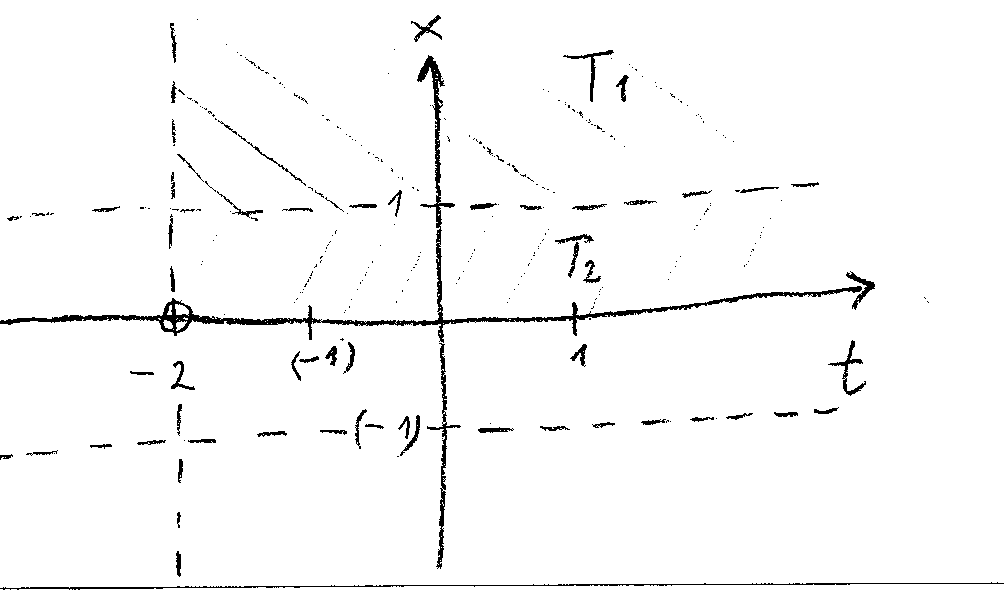
\includegraphics[width=0.52\linewidth]{tartomanyok_T1_T2.png}
\figlabel{A tartományok eredeti kéziratos szemléltetése; $T_1$ és $T_2$ jelölések (16. PDF-oldal).}
\end{center}

\subsubsection*{1. eset: $T_1=(-2,+\infty)\times(1,+\infty)$}
\begin{center}
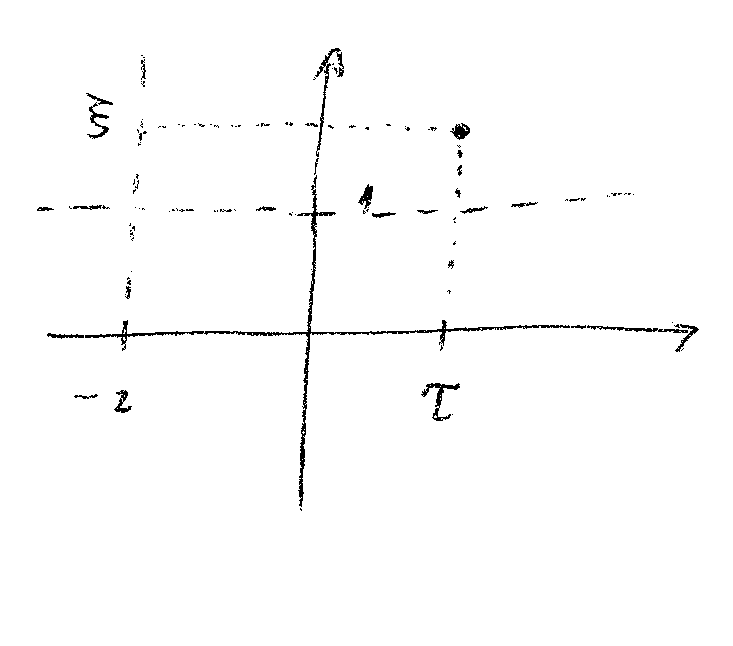
\includegraphics[width=0.36\linewidth]{kezdeti_adat_T1.png}
\figlabel{A $(\tau,\xi)$ kezdeti adat, $\xi>1$ (17. PDF-oldal).}
\end{center}

Tegyük fel, hogy $\varphi$ a teljes megoldás. A megoldás képlete:
\begin{equation}\label{eq:case1implicit}
    \int_{\xi}^{\varphi(t)}\frac{s}{s^2-1}\,ds
       =\int_{\tau}^{t}\frac{1}{2+s}\,ds,
       \qquad t\in\mathcal D_\varphi.
\end{equation}
\textbf{Megjegyzés.} A $\ln$ függvény komplex számokra is értelmezhető; lásd komplex függvénytan.

\begin{align*}
\Longrightarrow\quad
    \int_{\tau}^{t}\frac{1}{2+s}\,ds
       &=\ln(2+t)-\ln(2+\tau)
         =\ln\!\left(\frac{2+t}{2+\tau}\right),\\
    \int_{\xi}^{\varphi(t)}\frac{s}{s^2-1}\,ds
       &=\frac12\int_{\xi}^{\varphi(t)}2\cdot\frac{s}{s^2-1}\,ds\\
       &=\frac12\ln\!\left(\frac{\varphi^2(t)-1}{\xi^2-1}\right)
         =\ln\sqrt{\frac{\varphi^2(t)-1}{\xi^2-1}}\\
       &=\ln\!\left(\frac{2+t}{2+\tau}\right).
\end{align*}
Innen
\begin{equation}\label{eq:case1}
    \frac{\varphi^2(t)-1}{\xi^2-1}
      =\left(\frac{2+t}{2+\tau}\right)^2,
      \qquad t\in\mathcal D_\varphi.
\end{equation}

A teljes megoldás értelmezési tartománya:
\begin{align*}
 \inf_{u>1}\int_{\xi}^{u}\frac{1}{h(s)}\,ds
   &=\inf_{u>1}\frac12\ln\!\left(\frac{u^2-1}{\xi^2-1}\right)\\
   &=\frac12\inf_{u>1}\ln\!\left(\frac{u^2-1}{\xi^2-1}\right)=-\infty,\\
 \sup_{u>1}\cdots&=+\infty.
\end{align*}
\begin{align*}
\Longrightarrow\quad
 \mathcal D_\varphi
   &=\left\{t\in(-2,+\infty):
           -\infty<\int_{\tau}^{t}g<+\infty\right\}\\
   &=(-2,+\infty).
\end{align*}
Minden $(\tau,\xi)$ esetén a teljes megoldás értelmezési tartománya: $(-2,+\infty)$.

\textbf{A megoldások tulajdonságai.}
\begin{align*}
    \varphi'(t)&=\frac{1}{2+t}\cdot
       \frac{\varphi^2(t)-1}{\varphi(t)}>0,\\[-2pt]
    &\qquad t\in(-2,+\infty),\quad\varphi(t)\in(1,+\infty).
\end{align*}
\[
    \Longrightarrow\quad
    \varphi\ \text{szigorúan monoton növekvő }(-2,+\infty)\text{-en, és }
    \varphi\ \text{konvex is }(-2,+\infty)\text{-en (!)}.
\]
\[
    \lim_{t\to-2+0}\varphi(t)=1,
    \qquad \lim_{t\to+\infty}\varphi(t)=+\infty.
\]
\begin{center}
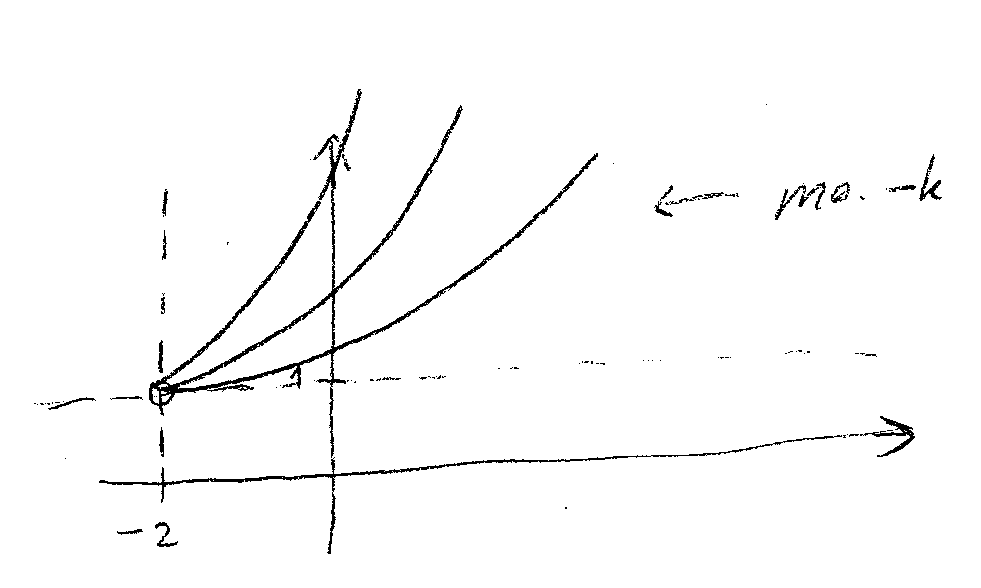
\includegraphics[width=0.53\linewidth]{megoldasgorbek_pozitiv.png}
\figlabel{A $T_1$ tartományhoz tartozó növekvő megoldásgörbék (18. PDF-oldal).}
\end{center}

\subsubsection*{2. eset: $T_2=(-2,+\infty)\times(0,1)$}
Előzőhöz hasonlóan figyeljük a teljes megoldás értelmezési tartományát.
\begin{center}
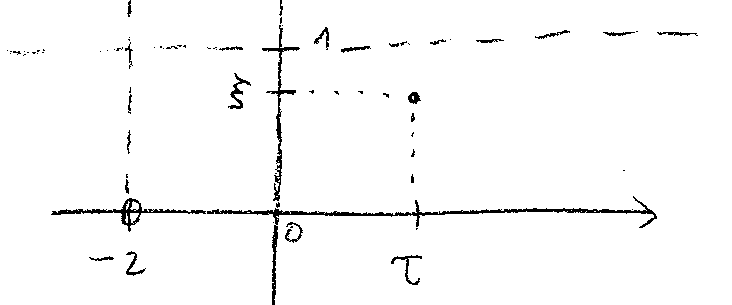
\includegraphics[width=0.38\linewidth]{kezdeti_adat_T2.png}
\figlabel{A $0<\xi<1$ kezdeti adat (18. PDF-oldal).}
\end{center}

Legyen $\varphi$ a teljes megoldás. A megoldás képlete:
\begin{equation}\label{eq:case2}
    \frac{1-\varphi^2(t)}{1-\xi^2}
        =\left(\frac{t+2}{\tau+2}\right)^2,
        \qquad t\in\mathcal D_\varphi.
\end{equation}
$\mathcal D_\varphi$ meghatározása:
\begin{align*}
  \inf_{0<u<1}\frac12\ln\!\left(\frac{1-u^2}{1-\xi^2}\right)
    &=-\infty,\\
  \sup_{0<u<1}\frac12\ln\!\left(\frac{1-u^2}{1-\xi^2}\right)
    &=\frac12\ln\!\left(\frac{1}{1-\xi^2}\right).
\end{align*}
\begin{align*}
 \Longrightarrow\qquad \mathcal D_\varphi
   &=\left\{t\in(-2,+\infty):
        -\infty<\ln\!\left(\frac{t+2}{\tau+2}\right)
         <\ln\!\left(\frac{1}{\sqrt{1-\xi^2}}\right)\right\}\\
   &=\left\{t\in(-2,+\infty):
          t+2<\frac{\tau+2}{\sqrt{1-\xi^2}}\right\}\\
   &\Longrightarrow\quad
     \mathcal D_\varphi=\left(-2,\frac{\tau+2}{\sqrt{1-\xi^2}}-2\right).
\end{align*}
A $\varphi$ függvény menete, határértéke:
\begin{center}
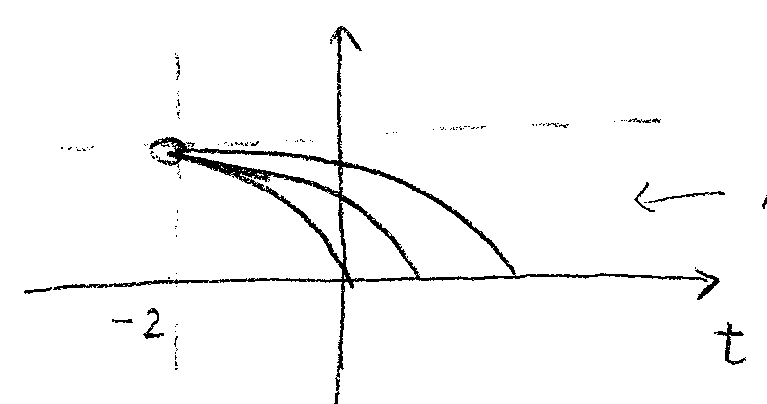
\includegraphics[width=0.42\linewidth]{megoldasgorbek_negativ.png}
\figlabel{A $T_2$-beli csökkenő megoldásgörbék (18. PDF-oldal).}
\end{center}

\begin{center}
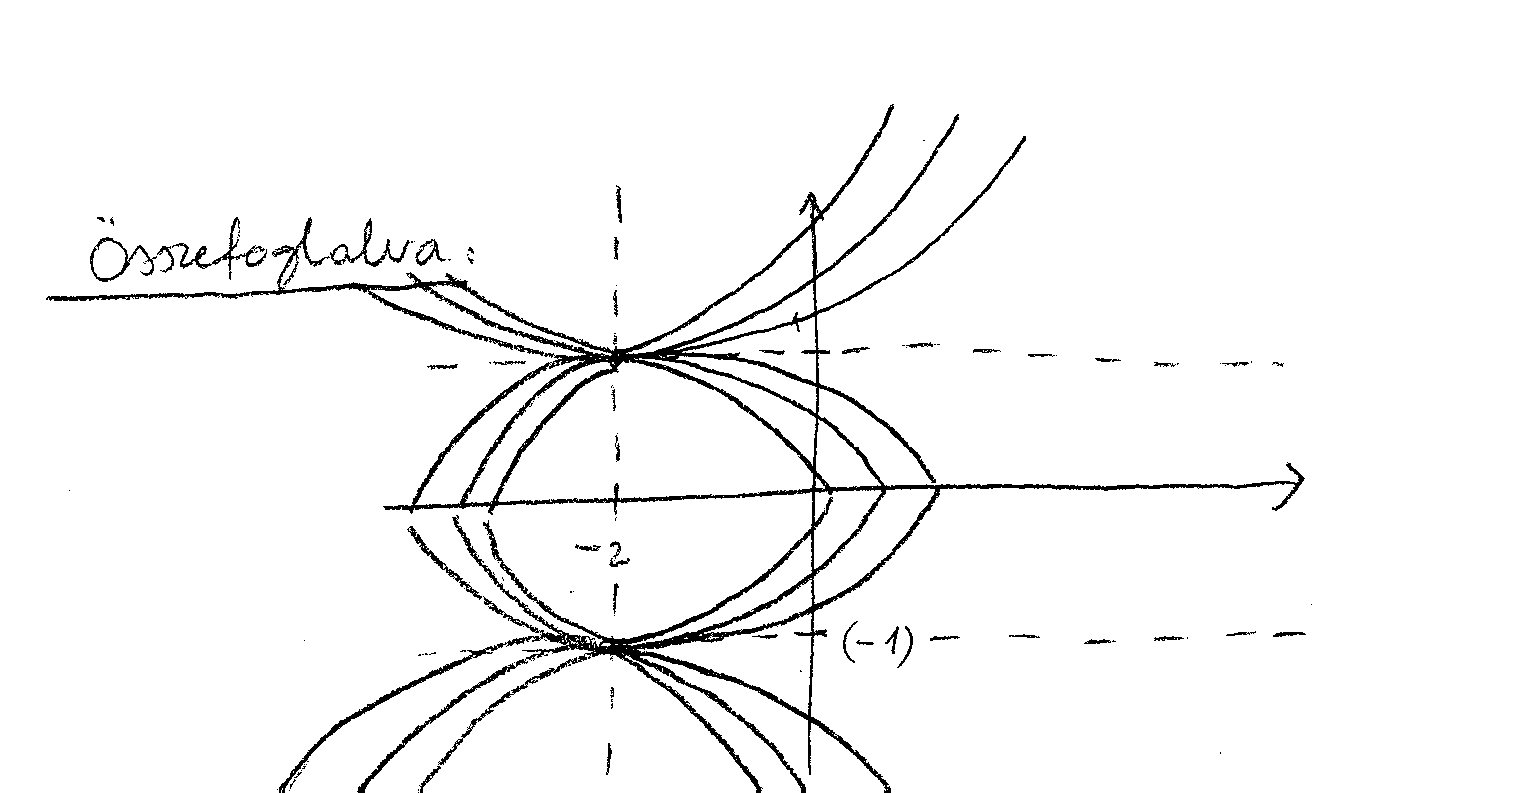
\includegraphics[width=0.57\linewidth]{megoldasgorbek_osszes.png}
\figlabel{A megoldásgörbék eredeti összefoglaló ábrája (18. PDF-oldal).}
\end{center}

\subsection{Szeparábilis differenciálegyenletre vezető típusok}
\textbf{1. típus.} Tegyük fel, hogy
\[
  f\in C([a,b],\mathbb R),\qquad\alpha,\beta,\gamma\in\mathbb R.
\]
\[
   x'(t)=f\bigl(\alpha t+\beta x(t)+\gamma\bigr).
\]
Legyen
\[
  u(t):=\alpha t+\beta x(t)+\gamma.
\]
Ekkor
\begin{equation*}
\Longrightarrow\qquad
   u'(t)=\alpha+\beta x'(t)
        =\alpha+\beta\,f(u(t)),
\end{equation*}
ami $u$-ra szétválasztható differenciálegyenlet.

\textbf{2. típus. Homogén fokszámú differenciálegyenlet.}
\[
   f\in C([a,b],\mathbb R),
   \qquad x'(t)=f\!\left(\frac{x(t)}{t}\right).
\]
\textit{(Folyt....)}
